\documentclass{article}

\usepackage[french]{babel}
\usepackage[utf8]{inputenc}
\usepackage[T1]{fontenc}
\usepackage[]{amsmath}
\usepackage{graphicx}
\usepackage{subcaption}
\usepackage{hyperref}
\usepackage{float}
\usepackage{amssymb}
\usepackage{setspace}

%%%%%%%%%%%%%%%% Lengths %%%%%%%%%%%%%%%%
\setlength{\textwidth}{15.5cm}
\setlength{\evensidemargin}{0.5cm}
\setlength{\oddsidemargin}{0.5cm}

%%%%%%%%%%%%%%%% Variables %%%%%%%%%%%%%%%%
\def\projet{5}
\def\titre{Interpolation and integration methods / cubic splines and surface interpolation}
\def\groupe{4}
\def\equipe{4}
\def\responsible{aguerouani}
\def\secretary{mrekik018}
\def\others{mchellaf, acattarin}
\newcommand{\summation}[2]{\sum\limits^{#1}_{#2}}

\begin{document}

%%%%%%%%%%%%%%%% Header %%%%%%%%%%%%%%%%
\noindent\begin{minipage}{0.98\textwidth}
  \vskip 0mm
  \noindent
  { \begin{tabular}{p{7.5cm}}
      {\bfseries \sffamily
        Projet \projet} \\ 
      {\itshape \titre}
    \end{tabular}}
  \hfill 
  \fbox{\begin{tabular}{l}
      {~\hfill \bfseries \sffamily Groupe \groupe\ - Equipe \equipe
        \hfill~} \\[2mm] 
      Responsable : \responsible \\
      Secrétaire : \secretary \\
      Codeurs : \others
    \end{tabular}}
  \vskip 4mm ~

  ~~~\parbox{0.95\textwidth}{\small \textit{This project focused on the study and implementation of interpolation and integration methods. This report discusses cubic spline interpolation and different integration methods. The objective was to compute a pressure map around the airfoil by using interpolation and integration} \sffamily }
  \vskip 1mm ~
\end{minipage}

%%%%%%%%%%%%%%%% Main part %%%%%%%%%%%%%%%%

\section{Airfoil refinement - Cubic spline}
\label{sec:cub_spline}
The first part of this project discusses the use of cubic spline interpolation. This algorithm was used to interpolate a series of points representing an airfoil. Between each point, the algorithm computed a polynomial with a degree at most 3. The final interpolation was a continuous function passing by all the points. This algorithm was implemented with the help of \emph{Numerical Recipes}. Figure \ref{fig:interp} below illustrates the results for known functions.

\begin{figure}[h]
  \centering
  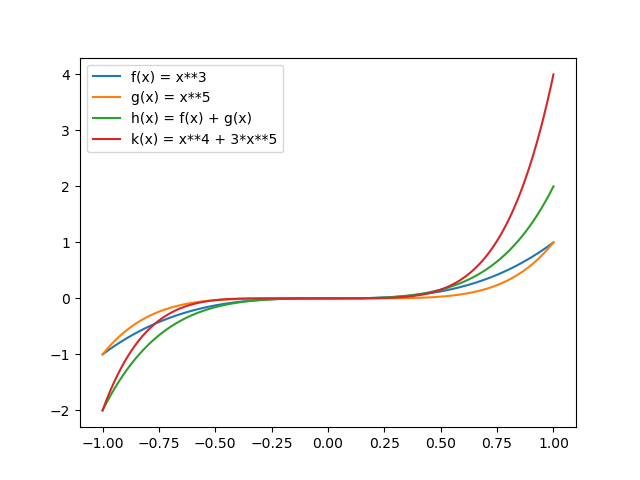
\includegraphics[width=0.45\textwidth]{img/interpolations.png}
  \caption{Cubic interpolations of known functions}
  \label{fig:interp}
\end{figure}

These results are visually significant as the curves look like the functions. This was also verified numerically.

\bigskip


Following that, the cubic spline algorithm was used to compute functions representing an airfoil. A series of points were given in a file. This algorithm was applied to these points, and a function was identified. This function and the points can be observed in Figure \ref{fig:airfoil}.

\begin{figure}[h]
  \centering
  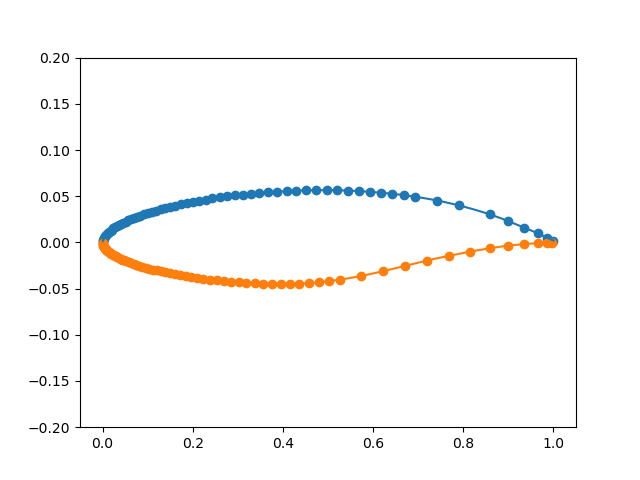
\includegraphics[width=0.45\textwidth]{img/airfoil_interp.png}
  \caption{Cubic interpolations of the airfoil}
  \label{fig:airfoil}
\end{figure}
  
This graph exhibits the links between all the points and the resultant function.

\bigskip

To use this algorithm, the boundary conditions were defined. Typically, the second derivatives at the first and last points are fixed at 0. In our implementation, the algorithm took the first derivatives and computed the second derivatives. To obtain the second derivatives equal to 0, the first derivatives had to be more than $10^{30}$.

The values of the first derivatives impacted the interpolation curves around the first and last points.


\section{Computing the length of plane curves - integration}
\label{sec:integr}
\large \emph{\textbf{Abdelhafid Guerouani}}

In this part, we have implemented five different integration methods to compute the length of plane curves defined by an integral. The objective is to optimize the measurement of the curves by choosing the appropriate method in terms of speed and convergence.
Selecting the right integration method is crucial for achieving accurate and efficient results. Therefore, we have tested and compared the performance of each method to determine which one is most suitable for our application.
\subsection{Integration methods}
Let $ f : [a,b] \rightarrow \mathbb{R} $, $n$ the number of intervals with $a = x_{0} < x_{1}< ...<x_{n} = b$ and $ h = x_{i+1} -x{i}$ the constant length of intervals.
\paragraph{left and right rectangle method}
The rectangle approximation method consists on dividing the area under a curve into multiple rectangles with small widths. This method is based on the Riemann integral definition and assumes that the widths of the rectangles are constant.
When computing a Riemann sum, the method for positioning the rectangles is important. One possibility is to align the rectangles such that their top-left corners touch the curve, which is referred to as a left Riemann sum given by $\int_{a}^{b}f(x)dx =  h\sum_{k=0}^{k=n-1} f(x_{k}) $.
Another approach is to place the rectangles such that their top-right corners touch the curve, known as a right Riemann sum and given by $\int_{a}^{b}f(x)dx =  h\sum_{k=1}^{k=n} f(x_{k}) $.
\paragraph{middle point method}
The middle point method is another option of the rectangle approximation which involves aligning the rectangles such that their midpoints touch the curves. This method is implemented by the following formula $\int_{a}^{b}f(x)dx =  h\sum_{k=1}^{k=n} f(\frac{x_{i-1} -x{i}}{2})$.
\paragraph{Trapezoidal method}
The trapezoidal method is a numerical integration technique that approximates the area under a curve by dividing the region into multiple trapezoids, rather than rectangles as in the rectangle method. By summing up the areas of all the trapezoids, we can obtain an estimation of the integral. Unlike the rectangle method, the trapezoidal method considers the slope of the curve between each pair of adjacent points by using a linear interpolation, which results in a more accurate approximation. The formula for trapezoidal method is :
$\int_{a}^{b}f(x)dx  = \frac{h}{2}(f(a) + f(b)) + h\sum_{k=1}^{k=n} f(x_{k}) = I_{h}$

\paragraph{Simpson method}
Simpson's method is a numerical integration technique that approximates the area under a curve by dividing the region into an even number of subintervals and fitting a second-degree polynomial to each pair of consecutive points on the curve. By computing the area under each parabolic segment and summing them up, we can obtain an estimation of the integral. Simpson's method is known to be more accurate than the rectangle and trapezoidal methods, especially for curves that are quadratic or less, as it can provide exact results in such cases. The formula for Simpson's method is : \\
$\int_{a}^{b}f(x)dx = \frac{h}{6}(f(a)+f(b)) +\frac{2h}{3}\sum_{k=0}^{k=n-1}f(x_{i} +\frac{h}{2})  + \frac{h}{3}\sum_{k=0}^{k=n-1} f(x_{i}) = \frac{4}{3}I_{\frac{h}{2}} - \frac{1}{3}I_{h} $ \\
with $I_{h}$ the trapezoidal approximation of $\int_{a}^{b}f(x)dx $ using $\frac{a-b}{h}$ interval.

\subsection{Convergence analysis}
\label{section}
Once we validated the different integration methods on various polynomial and non-polynomial functions, we proceeded to analyze their convergence for a specific polynomial integral $ I = \int_{0}^{2}(x^{3} -3x +2)dx$. To do so, we evaluated the integral approximation for different values of the number $N$ of intervals, and studied how the accuracy of the approximation improved as we increased $N$. \\
According to Figure \ref{fig:speed}, the Simpson's method displays a faster convergence than the trapezoidal and rectangle methods. In fact, for $N=10$, the Simpson's method achieves an error of about $10^{-16}$, while the trapezoidal method yields an error of $0.04$, and the midpoint method yields an error of $0.01$. On the other hand, the left and right rectangle methods converge much more slowly.These results could be justified by the fact that the Simpson's method approximates the curve with quadratic polynomials, while the other methods use linear approximations.\\
\begin{figure}[h]
  \centering
  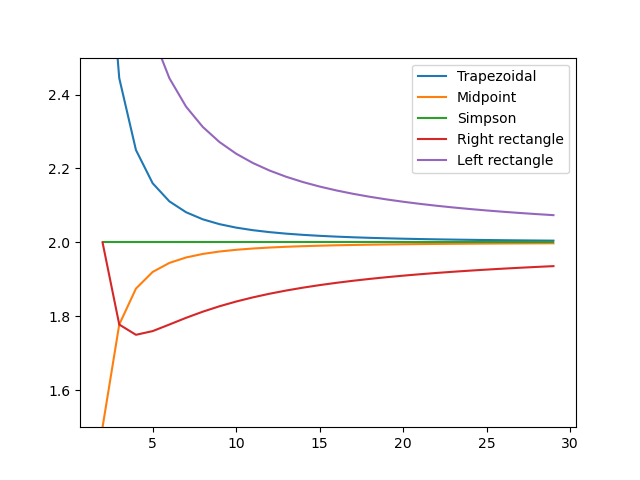
\includegraphics[width=0.45\textwidth]{img/speed_convergence.png}
  \caption{Approximations of the integral in function of the number $N$ of intervals I using the different methods}
  \label{fig:speed}
\end{figure}

\subsection{Length of the plane curves} 
In section~\ref{section}, it was found that the Simpson method is a suitable numerical integration method for approximating the length of splines, as it provides fast convergence and high accuracy. This method can be used to approximate the integral $\int \sqrt{1+f'(x)^{2}}dx$, which is used to determine the length of the spline.

To approximate the derivative of the function f, we utilized the central difference formula $f'(x) = \frac{f'(x+h) - f'(x-h)}{2h}$, which uses the values of the function at points slightly to the left and right of the point at which the derivative is being approximated. This formula has an error of order 2, which means that the accuracy of the approximation improves as the step size h becomes smaller.




\section{Modelling the airflow / Pressure map}
\label{sec:press_map}
\subsection{Modelling the airflow}
\large \emph{\textbf{Mohamed Rekik}}

In the field of aerodynamics, modeling the airflow around an object such as an airplane wing is crucial to understanding its performance. In this particular case, the airflow around a previously interpolated wing will be modeled using a laminar flow assumption. Laminar flow means that the airflow can be divided into two parts, and each air molecule moves along curves that do not intersect. This is an important assumption because it simplifies the modeling process and allows for more accurate predictions.

To model the airflow, the minimum and maximum height of the airflow were first determined to be $h_{min}^{m}$ and $h_{max}^{m}$, respectively. The airflow is assumed to be disturbed by the wing in a vertical interval of $[[3h_{min}; 3h_{max}]]$, while it is rectilinear elsewhere. This assumption is necessary to accurately capture the effect of the wing on the airflow.

The next step is to model the curve $y$ for either the extrados or the intrados. The curve $y$ represents the shape of the upper or lower surface of the wing. This is done using the equation given in (\ref{eq:equation_part3.1}), where $f(x)$ is the function that interpolates the points of the wing, and $\lambda$ is a parameter that varies between 0 and 1. The value of $\lambda$ determines the shape of the curve, with a value of 0 resulting in the original shape of the wing and a value of 1 resulting in a straight line at a height of $h_{max}\times 3$. By varying $\lambda$ between 0 and 1, the shape of the wing can be smoothly transitioned from its original shape to a straight line.
\begin{equation}
  \label{eq:equation_part3.1}
  y = f_{\lambda}(x) = (1 - \lambda)f(x) + \lambda \times h_{max} \times 3 \quad \forall \lambda \in [0,1] 
\end{equation}

To confirm the laminar nature of the airflow, several measurements are taken. These include the extrados $x/y$ $(ex, ey)$, the intrados $x/y$ $(ix, iy)$, the function that interpolates the points of the upper part of the wing (fint\_upp), and the function that interpolates the points of the lower part of the wing (fint\_low). A figure is obtained (see Figure \ref{fig:laminar}), which confirms the laminar nature of the airflow. The figure shows that the airflow above and below the wing follows a smooth and regular pattern, which is indicative of laminar flow.
\begin{figure}[H]
  \centering
  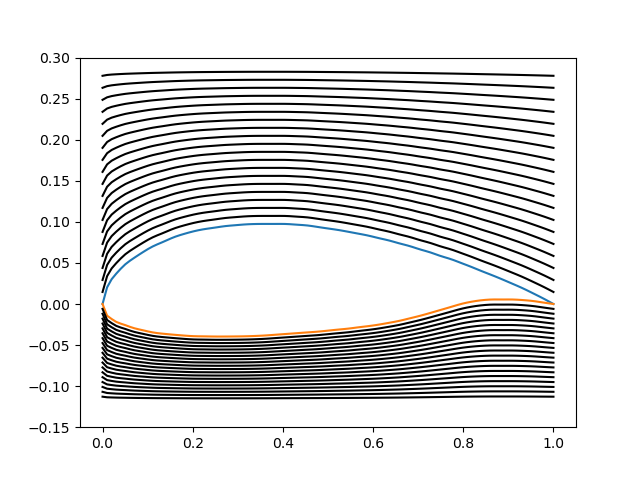
\includegraphics[width=0.45\textwidth]{img/laminar_flow.png}
  \caption{Laminar flow above and below the wing}
  \label{fig:laminar}
\end{figure}

In conclusion, modeling the airflow around a wing is an important step in understanding its performance. By assuming laminar flow and using various measurements, the shape of the airflow can be accurately predicted. This information is crucial for designing and optimizing airplane wings, and can lead to improved performance and efficiency.

\subsection{Pressure map}
\large \emph{\textbf{Mohamed Dyae Chellaf}}

As in the first subsection, we will use functions defined in the previous sections to approach the study of this subsection.
We must plot the function corresponding to the pressure distribution around the wing to have even more information on the aerodynamic profile and thus improve performance and characteristics.\\
We can ultimately come to understand the behavior of the air around the airfoil.\\
Given a laminar airflow, the particles move along independent trajectories.\\
In this sequence, we base ourselves on the distribution of the pressure in the surface of the aerodynamic profile drawn and we save the results.\\
And so does the pressure map obteined shows the informations about the airflow around the airfoil, and shows that the air moves more easily above the wing than below, which leads to a remarkable pressure difference, which in turn creates a lift force that gives the plane the ability to stay aloft?\\
\begin{figure}[h]
  \centering
  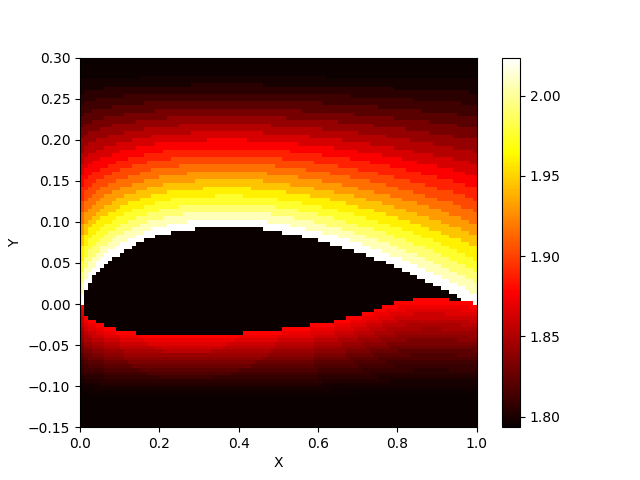
\includegraphics[width=0.45\textwidth]{img/pressure_map.png}
  \caption{Pressure map}
  \label{fig:pressure}
\end{figure}



\section{Conclusion}
\label{sec:ccl}
\large \emph{\textbf{Antton Cattarin}}

In this project, interpolation and integration methods were explored, specifically cubic splines and several numerical integration techniques. The results obtained from these methods were proven to be visually significant and numerically reliable.

The use of cubic splines allowed the interpolation of a series of points representing an airfoild, resulting in a continuous function passing through all the points.

Regarding the integration methods, five different techniques were implemented and tested, so the length of plane curves was measured. Each method was evaluated in terms of speed and convergence. The results obtained were found to be reliable.

Overall, these methods were proven to be useful in the numerical analysis of functions and curves. They allowed the accurate interpolation and integration of a series of points, leading to a trustworthy pressure map.


\end{document}
